\documentclass[10pt,journal]{IEEEtran}
\usepackage{cite}
\usepackage{amsmath,amssymb,amsfonts}
\usepackage{algorithmic}
\usepackage{graphicx}
\usepackage{textcomp}
\usepackage{booktabs}
\usepackage{url}
\usepackage{tikz}
\usetikzlibrary{positioning,arrows.meta}

\newcommand{\vect}[1]{\mathbf{#1}}
\newcommand{\mat}[1]{\mathbf{#1}}

\begin{document}

\title{Vision-Based Hand Shadowing for Robotic Manipulation via Inverse Kinematics}

\author{Hendrik Chiche, Antoine Jamme, and Trevor Rigoberto Martinez%
\thanks{Hendrik Chiche and Antoine Jamme are with OMGrab Inc. and affiliated with the University of California, Berkeley through the Capstone Project program (e-mail: hendrik\_chiche@berkeley.edu; antoine\_jamme@berkeley.edu). Trevor Rigoberto Martinez is with the Department of Mechanical Engineering, University of California, Berkeley (e-mail: tre\_mart@berkeley.edu).}%
}

\begin{abstract}
Teleoperation of low-cost robotic manipulators remains challenging due to the
complexity of mapping human hand articulations to robot joint commands.
We present an offline hand-shadowing and retargeting pipeline from a
single egocentric RGB-D camera mounted on 3D-printed glasses. The pipeline
detects 21 hand landmarks per hand using MediaPipe Hands, deprojects them
into 3D via depth sensing, transforms them into the robot coordinate frame,
and solves a damped-least-squares inverse kinematics problem in PyBullet to
produce joint commands for the 6-DOF SO-ARM101 robot. A gripper controller
maps thumb--index finger geometry to grasp aperture with a four-level
fallback hierarchy. Actions are first previewed in a physics simulation
before replay on the physical robot through the LeRobot framework.
We evaluate the IK retargeting pipeline on a structured pick-and-place
benchmark (5-tile grid, 10 grasps per tile) achieving a 90\% success rate,
and compare it against four vision-language-action policies
(ACT, SmolVLA, $\pi_{0.5}$, GR00T~N1.5) trained on
leader--follower teleoperation data. We also test the IK pipeline
in unstructured real-world environments (grocery store, pharmacy),
where hand occlusion by surrounding objects reduces success to
9.3\% ($N=75$), highlighting both the promise and current limitations
of marker-free analytical retargeting.
\end{abstract}

\begin{IEEEkeywords}
Hand tracking, inverse kinematics, MediaPipe, PyBullet, robot teleoperation,
retargeting, SO-ARM101, vision-language-action models.
\end{IEEEkeywords}

\maketitle

\begin{center}
\begin{minipage}{0.98\linewidth}
\footnotesize
\raggedright
\textit{Project resources:}\\
Video demonstration: \url{https://youtu.be/mKtVg_gYwf8}\\
Datasets and fine-tuned models: \url{https://huggingface.co/Chichonnade}\\
Source code: \url{https://github.com/chichonnade/Vision-Based-Hand-Shadowing}
\end{minipage}
\end{center}

% ============================= 1  INTRODUCTION ==============================
\section{Introduction}
\label{sec:introduction}
Teaching robots to manipulate objects the way humans do is a
central goal of robotics research. Two dominant paradigms have emerged:
\emph{teleoperation}, where a human operator directly controls the robot
in real time, and \emph{imitation learning}, where a policy is trained
from recorded demonstrations~\cite{zhao2023act,cadena2025smolvla}.
Teleoperation provides immediate, interpretable control but traditionally
requires expensive hardware such as exoskeletons, leader--follower arm
pairs, or VR headsets~\cite{cheng2025opentv,ding2024bunny}. Imitation
learning can reduce the demonstration burden but demands careful data
collection, GPU-based training, and policy evaluation.

This work studies how an analytical inverse-kinematics pipeline can
bridge these paradigms by converting first-person RGB-D recordings into
robot trajectories that can be replayed on hardware and reused as
training data for imitation-learning frameworks.
Our contributions are:

\begin{enumerate}
  \item An end-to-end pipeline from egocentric RGB-D video
        to single-arm robot trajectory generation via analytical inverse
        kinematics.
  \item A sim-to-real transfer workflow using PyBullet for trajectory
        preview and validation before physical deployment on the
        SO-ARM101 robot.
  \item A quantitative comparison of analytical IK retargeting with
        four VLA policies on a structured pick-and-place benchmark.
  \item An in-the-wild evaluation in grocery store and pharmacy
        environments to assess robustness under clutter and occlusion.
\end{enumerate}

Across these studies, the IK pipeline reaches 90\% success on the
structured benchmark with zero training, while hand occlusion emerges as
the main limitation in unstructured scenes.

% ============================= 2  RELATED WORK ==============================
\section{Related Work}
\label{sec:related}

\subsection{Hand Pose Estimation}
Real-time hand tracking has advanced rapidly. MediaPipe
Hands~\cite{zhang2020mediapipe} runs on-device at 30\,Hz using a
two-stage BlazePalm + landmark pipeline predicting 21 keypoints,
and requires no GPU. We adopt MediaPipe for its CPU efficiency and
cross-platform availability.
WiLoR~\cite{potamias2024wilor} improves accuracy with a DarkNet
localiser followed by a ViT-based 3D reconstructor, achieving
state-of-the-art results on FreiHAND and HO3D benchmarks at over
130\,FPS but requires GPU inference. Both systems output 21 keypoints
compatible with the MANO hand model topology~\cite{romero2017mano}.

\subsection{Teleoperation Systems}
Open-TeleVision~\cite{cheng2025opentv} provides stereoscopic VR-based
teleoperation for humanoid robots. Bunny-VisionPro~\cite{ding2024bunny}
uses Apple Vision Pro for bimanual dexterous control with haptic
feedback. These systems achieve high fidelity but require specialised
VR hardware. Our approach uses only an RGB-D depth camera and
3D-printed accessories.

\subsection{Imitation Learning}
ACT~\cite{zhao2023act} introduced action chunking with transformers for
fine-grained bimanual manipulation, achieving 80--90\% success with
10 minutes of demonstrations. SmolVLA~\cite{cadena2025smolvla} is a
450M-parameter vision-language-action model trainable on a single GPU.
$\pi_0$~\cite{black2024pi0} is a generalist robot foundation model
using flow matching over a VLM backbone, trained across 7 robot
embodiments and 68 tasks.

\subsection{Low-Cost Robotics}
The SO-ARM100/101 is a 6-DOF arm using STS3215 bus servos
with 30\,kg$\cdot$cm torque~\cite{soarm100}. LeRobot~\cite{lerobot2024}
provides a hardware-agnostic Python framework that standardises data
collection, training, and deployment across robot platforms.

\subsection{Physics Simulation}
PyBullet~\cite{coumans2021pybullet} provides real-time rigid body
dynamics with built-in inverse kinematics via the Bullet Physics SDK.
It supports URDF loading, position/velocity/torque control, and
GPU-accelerated rendering, making it suitable for rapid prototyping
and sim-to-real transfer.

% ============================= 3  SYSTEM OVERVIEW ===========================
\section{System Overview}
\label{sec:system}

The system converts egocentric hand observations into robot
commands through a multi-stage transformation pipeline
(Fig.~\ref{fig:architecture}). It requires an Intel RealSense
D400 camera~\cite{keselman2017realsense} mounted on 3D-printed glasses
and a single SO-ARM101 follower arm. At the software level, each
pipeline stage is implemented as a \texttt{Transformation[InT, OutT]}
subclass that wraps a \texttt{\_transform} method with automatic
latency tracking.

Table~\ref{tab:pipeline} lists each stage with its input and output
types; Fig.~\ref{fig:architecture} shows the overall data flow.

\begin{figure}[t]
\centering
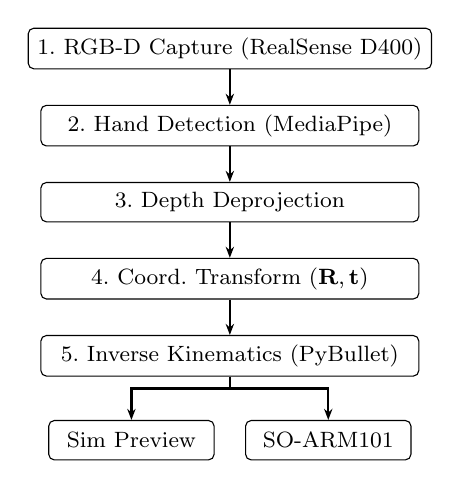
\begin{tikzpicture}[
  node distance=0.45cm,
  stage/.style={rectangle, draw, rounded corners=2pt,
    minimum width=4.8cm, minimum height=0.5cm,
    align=center, font=\footnotesize},
  output/.style={rectangle, draw, rounded corners=2pt,
    minimum width=2.1cm, minimum height=0.5cm,
    align=center, font=\footnotesize},
  arr/.style={-{Stealth[length=4pt]}, thick}
]
\node[stage] (cam)   {1.~RGB-D Capture (RealSense D400)};
\node[stage, below=of cam]   (hand)  {2.~Hand Detection (MediaPipe)};
\node[stage, below=of hand]  (depth) {3.~Depth Deprojection};
\node[stage, below=of depth] (coord) {4.~Coord.\ Transform ($\mathbf{R},\mathbf{t}$)};
\node[stage, below=of coord] (ik)    {5.~Inverse Kinematics (PyBullet)};
\node[output, below=0.55cm of ik, xshift=-1.25cm] (sim)   {Sim Preview};
\node[output, below=0.55cm of ik, xshift=1.25cm]  (robot) {SO-ARM101};
\draw[arr] (cam)   -- (hand);
\draw[arr] (hand)  -- (depth);
\draw[arr] (depth) -- (coord);
\draw[arr] (coord) -- (ik);
\draw[arr] (ik.south) -- ++(0,-0.15) -| (sim.north);
\draw[arr] (ik.south) -- ++(0,-0.15) -| (robot.north);
\end{tikzpicture}
\caption{\textbf{System architecture.} The six-stage pipeline converts
  egocentric RGB-D observations into robot joint commands. Stages 1--5
  run sequentially; the output drives either the PyBullet simulation
  for preview or the physical SO-ARM101 for deployment.}
\label{fig:architecture}
\end{figure}

\begin{table}[t]
\caption{\textbf{Pipeline Stages With Input/Output Types}}
\label{tab:pipeline}
\centering
\begin{tabular}{clll}
\hline
\textbf{\#} & \textbf{Stage} & \textbf{Input} & \textbf{Output} \\
\hline
1 & Camera Input        & None         & CameraFrame \\
2 & Hand Detection      & CameraFrame  & ImageSpace \\
3 & Depth Deprojection  & (ImageSpace, & CameraSpace \\
  &                     & \ CameraFrame) & \\
4 & Coord.\ Transform   & CameraSpace  & RobotSpace \\
5 & IK + Gripper        & RobotSpace   & ControlCmds \\
6 & Sim / Robot         & ControlCmds  & --- \\
\hline
\end{tabular}
\end{table}

\subsection{Hardware}
\label{sec:hardware}

The egocentric sensor platform consists of an Intel RealSense D400-series
stereo depth camera mounted on 3D-printed glasses using three PLA/ABS
parts (frame, two temple branches, and a camera mount bracket), secured
with M1.5, M2, and M3 screws. The camera connects via USB-C 3.1 Gen~1
and streams synchronised RGB and depth at 640$\times$480 resolution and
30\,FPS. The robot platform uses a single SO-ARM101 follower arm
with 6 revolute joints (5 arm + 1 gripper) driven by STS3215
Feetech bus servos. The complete lab bench setup, including the robot
and egocentric camera stand, is shown in Fig.~\ref{fig:bench}.

\begin{figure}[t]
\centering
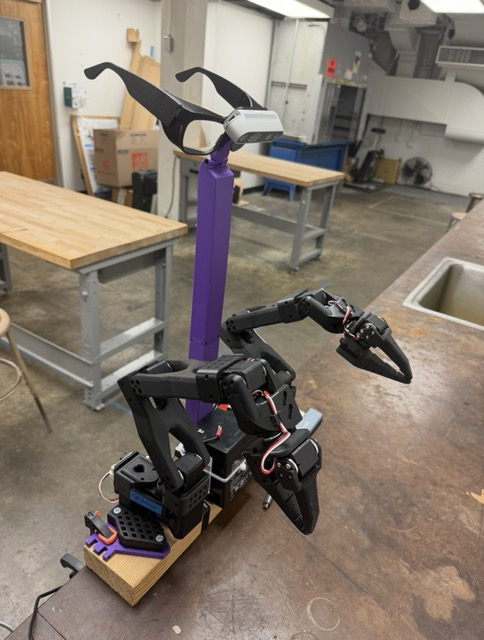
\includegraphics[width=0.9\columnwidth]{robot.JPG}
\caption{\textbf{Lab bench setup.} The SO-ARM101 robot arm is mounted on a
  wooden base with the Intel RealSense D400 camera on a stand above,
  oriented in the same egocentric direction as the glasses-mounted camera.}
\label{fig:bench}
\end{figure}

% ============================= 4  METHODS ===================================
\section{Methods}
\label{sec:methods}

\subsection{RGB-D Capture and Camera Model}
\label{sec:camera}

The RealSense camera provides aligned RGB-D frames via the
\texttt{pyrealsense2} SDK. We model the camera using the pinhole
projection:
\begin{equation}\label{eq:projection}
  \begin{bmatrix} u \\ v \end{bmatrix}
  = \begin{bmatrix} f_x & 0 & c_x \\ 0 & f_y & c_y \end{bmatrix}
    \begin{bmatrix} X/Z \\ Y/Z \\ 1 \end{bmatrix},
\end{equation}
where $(f_x, f_y)$ are focal lengths and $(c_x, c_y)$ is the principal
point, all extracted automatically from the camera stream at
initialisation. The camera supports recording to \texttt{.bag} files for
offline processing and to MP4 for archival.

\subsection{Hand Pose Estimation}
\label{sec:handpose}

We use MediaPipe Hands~\cite{zhang2020mediapipe} for 2D hand detection
and landmark localisation. MediaPipe's two-stage architecture---a
BlazePalm detector that locates hands via oriented bounding boxes,
followed by a lightweight landmark regression network---predicts
21 keypoints per hand in real time on CPU. The detector outputs
left/right hand classification and 2D keypoint coordinates
$\{(u_i, v_i)\}_{i=0}^{20}$ covering the wrist, thumb, index, middle,
ring, and pinky finger joints.

To reduce temporal jitter, we apply exponential moving average (EMA)
smoothing to the 2D landmarks:
\begin{equation}\label{eq:ema}
  \hat{p}_t = \alpha\, p_t + (1 - \alpha)\, \hat{p}_{t-1},
  \quad \alpha = 0.8,
\end{equation}
where $p_t$ is the raw detection and $\hat{p}_t$ is the smoothed
estimate.

\subsection{Depth-Based 3D Reconstruction}
\label{sec:depth3d}

Each 2D landmark $(u_i, v_i)$ is deprojected to 3D camera coordinates
using the depth image $D$ and camera intrinsics:
\begin{equation}\label{eq:deproject}
  \begin{bmatrix} X \\ Y \\ Z \end{bmatrix}
  = \frac{D[v_i, u_i]}{s}
    \begin{bmatrix}
      (u_i - c_x) / f_x \\
      (v_i - c_y) / f_y \\
      1
    \end{bmatrix},
\end{equation}
where $s = 1000$ is the depth scale (millimetres to metres). Depth
values are validated against the range $[d_{\min}, d_{\max}] =
[0.1, 5.0]$\,m; landmarks with out-of-range depth are marked invalid.

A \emph{depth fallback} mechanism handles the critical case where one of
the two gripper-defining landmarks (THUMB\_MCP or INDEX\_FINGER\_MCP)
has invalid depth but the other does not. In this case, the valid
landmark's depth is substituted for the failed one, since these adjacent
landmarks are typically at similar depths. A hand pose is rejected
entirely if fewer than 50\% of its 21 landmarks have valid depth.


\subsection{Camera-to-Robot Coordinate Transform}
\label{sec:transform}

Landmarks in camera coordinates $\vect{p}_{\text{cam}}$ are transformed
to the robot base frame $\vect{p}_{\text{rob}}$ by a rigid-body
transformation composed of a camera-to-robot transform and an optional
URDF offset:
\begin{equation}\label{eq:transform}
  \vect{p}_{\text{rob}} = \mat{R}_{\text{final}}\,\vect{p}_{\text{cam}}
                          + \vect{t}_{\text{final}},
\end{equation}
where
\begin{equation}
  \mat{R}_{\text{final}} = \mat{R}_{\text{urdf}} \cdot \mat{R}_{\text{cam}},
  \quad
  \vect{t}_{\text{final}} = \mat{R}_{\text{urdf}} \cdot \vect{t}_{\text{cam}}
                             + \vect{t}_{\text{urdf}}.
\end{equation}

The camera rotation matrix $\mat{R}_{\text{cam}}$ accounts for the
camera mounting angle $\theta = 50^{\circ}$:
\begin{equation}\label{eq:Rcam}
  \mat{R}_{\text{cam}} =
  \begin{bmatrix}
    -1 & 0 & 0 \\
    0 & \sin\theta & -\cos\theta \\
    0 & -\cos\theta & -\sin\theta
  \end{bmatrix},
\end{equation}
with translation $\vect{t}_{\text{cam}} = (0.04,\; -0.049,\; 0.48)^\top$
metres. These parameters---including the $50^{\circ}$ mounting angle and
translation offsets---are extracted directly from the SolidWorks CAD
assembly that models both the robot and the camera mount bracket at
their exact physical positions.
The $x$-axis negation mirrors the image horizontally (the camera
observes hands from a first-person perspective, while the robot faces
the operator), and the rotation about the $x$-axis maps the downward
camera view to the robot's forward--up coordinate system.

\subsection{Target Pose Computation}
\label{sec:targetpose}

The robot end-effector target position is the midpoint of the two
gripper-defining hand landmarks:
\begin{equation}\label{eq:targetpos}
  \vect{p}_{\text{target}} = \frac{1}{2}
    \bigl(\vect{p}_{\text{THUMB\_MCP}} +
    \vect{p}_{\text{INDEX\_FINGER\_MCP}}\bigr).
\end{equation}

The target orientation is constructed as a rotation matrix from three
orthogonal axes derived from hand geometry:
\begin{align}
  \vect{e}_1 &= \frac{\vect{p}_{\text{INDEX\_FINGER\_MCP}} -
    \vect{p}_{\text{THUMB\_MCP}}}
    {\|\vect{p}_{\text{INDEX\_FINGER\_MCP}} -
    \vect{p}_{\text{THUMB\_MCP}}\|},
    \label{eq:e1} \\
  \vect{d} &= \frac{1}{2}\bigl(
    (\vect{p}_{\text{THUMB\_TIP}} - \vect{p}_{\text{THUMB\_MCP}}) \nonumber \\
    &\quad + (\vect{p}_{\text{INDEX\_FINGER\_TIP}} -
    \vect{p}_{\text{INDEX\_FINGER\_MCP}})
  \bigr), \label{eq:avgdir} \\
  \hat{\vect{d}} &= \frac{\vect{d}}{\|\vect{d}\|}, \nonumber \\
  \vect{e}_3 &= \frac{\vect{e}_1 \times \hat{\vect{d}}}
    {\|\vect{e}_1 \times \hat{\vect{d}}\|}, \label{eq:e3} \\
  \vect{e}_2 &= \vect{e}_3 \times \vect{e}_1. \label{eq:e2}
\end{align}
The resulting rotation matrix $\mat{R} = [\vect{e}_1 \;\; \vect{e}_2
\;\; \vect{e}_3]$ is converted to a quaternion via
\texttt{scipy.spatial.transform} for the IK solver.

When fingertip landmarks are unavailable (due to occlusion or depth
failure), a \emph{fallback orientation} is computed using only
THUMB\_MCP, INDEX\_FINGER\_MCP, and WRIST, replacing the average finger
direction $\vect{d}$ with the wrist-to-gripper vector.

\subsection{Inverse Kinematics}
\label{sec:ik}

Given the target position $\vect{p}_{\text{target}}$ and orientation
quaternion $\vect{q}_{\text{target}}$, we solve for joint angles
$\vect{\theta} = (\theta_1, \ldots, \theta_5)$ of the 5-DOF arm using
PyBullet's \texttt{calculateInverseKinematics}:
\begin{equation}\label{eq:ik}
  \vect{\theta}^* = \arg\min_{\vect{\theta}}
  \bigl\|
    \text{FK}(\vect{\theta}) - (\vect{p}_{\text{target}},
                                  \vect{q}_{\text{target}})
  \bigr\|^2
  + \lambda \|\vect{\theta} - \vect{\theta}_{\text{rest}}\|^2,
\end{equation}
where $\text{FK}(\cdot)$ is the forward kinematics function,
$\vect{\theta}_{\text{rest}}$ is the current joint state (used as the
rest pose), and $\lambda$ captures per-joint damping extracted from the
URDF (clamped to $\geq 0.001$ to prevent solver instability). The solver
runs up to 100 iterations with a residual threshold of $10^{-4}$.

EMA smoothing ($\alpha = 0.5$) is applied to the IK solution to
suppress temporal jitter:
\begin{equation}
  \hat{\vect{\theta}}_t = 0.5\,\vect{\theta}^*_t
                        + 0.5\,\hat{\vect{\theta}}_{t-1}.
\end{equation}

A safety check rejects any target with $z < 0.05$\,m to prevent
ground-plane collisions.

\subsection{Gripper Control}
\label{sec:gripper}

The gripper angle $\phi$ is computed from the angular separation between
vectors from the gripper base (target position) to the thumb and index
finger:
\begin{equation}\label{eq:gripper}
  \phi = \arccos\!\left(
    \frac{(\vect{p}_{\text{thumb}} - \vect{p}_{\text{target}})
          \cdot
          (\vect{p}_{\text{index}} - \vect{p}_{\text{target}})}
         {\|\vect{p}_{\text{thumb}} - \vect{p}_{\text{target}}\|\;
          \|\vect{p}_{\text{index}} - \vect{p}_{\text{target}}\|}
  \right),
\end{equation}
clamped to the acute range $[0, \pi/2]$ and then to the gripper joint
limits $[\phi_{\min}, \phi_{\max}] = [0.087, 1.658]$\,rad after
applying an offset of $-0.175$\,rad for tighter grip calibration.

A four-level fallback hierarchy ensures robust gripper control:
\begin{enumerate}
  \item Use THUMB\_TIP and INDEX\_FINGER\_TIP (primary).
  \item Use THUMB\_IP and INDEX\_FINGER\_DIP (knuckle fallback).
  \item Use the last valid gripper angle (temporal persistence).
  \item Use the mid-open default $(\phi_{\min}+\phi_{\max})/2$.
\end{enumerate}

\subsection{Simulation Preview}
\label{sec:simulation}

Before deploying on the physical robot, all IK-generated trajectories
are previewed in a PyBullet simulation environment. The simulation
loads the SO-ARM101 URDF with 7 joints per arm
(1 fixed base + 5 revolute arm + 1 revolute gripper); only the
right arm is used in our experiments. The simulation
runs at 240\,Hz with gravity $g = 9.81$\,m/s$^2$. Joint commands
are executed via position control with uniform force limits of 6.0\,N,
position gains of 0.2, and velocity gains of 1.0.

Fig.~\ref{fig:simulation} shows the simulation preview interface.
The top-left panel displays the RGB frame from the egocentric
camera with the operator's hand visible; the top-right panel shows the
corresponding depth map colour-coded by distance; and the bottom panel
renders the robot in PyBullet tracking the hand-derived IK
targets. This three-panel view allows the operator to
verify that the computed joint trajectories faithfully reproduce the
intended hand motion before committing to physical execution.
Beyond trajectory verification, the simulation also exports
demonstration data (\texttt{.npy} action files) that can be used
to train imitation-learning policies.

\begin{figure}[t]
\centering
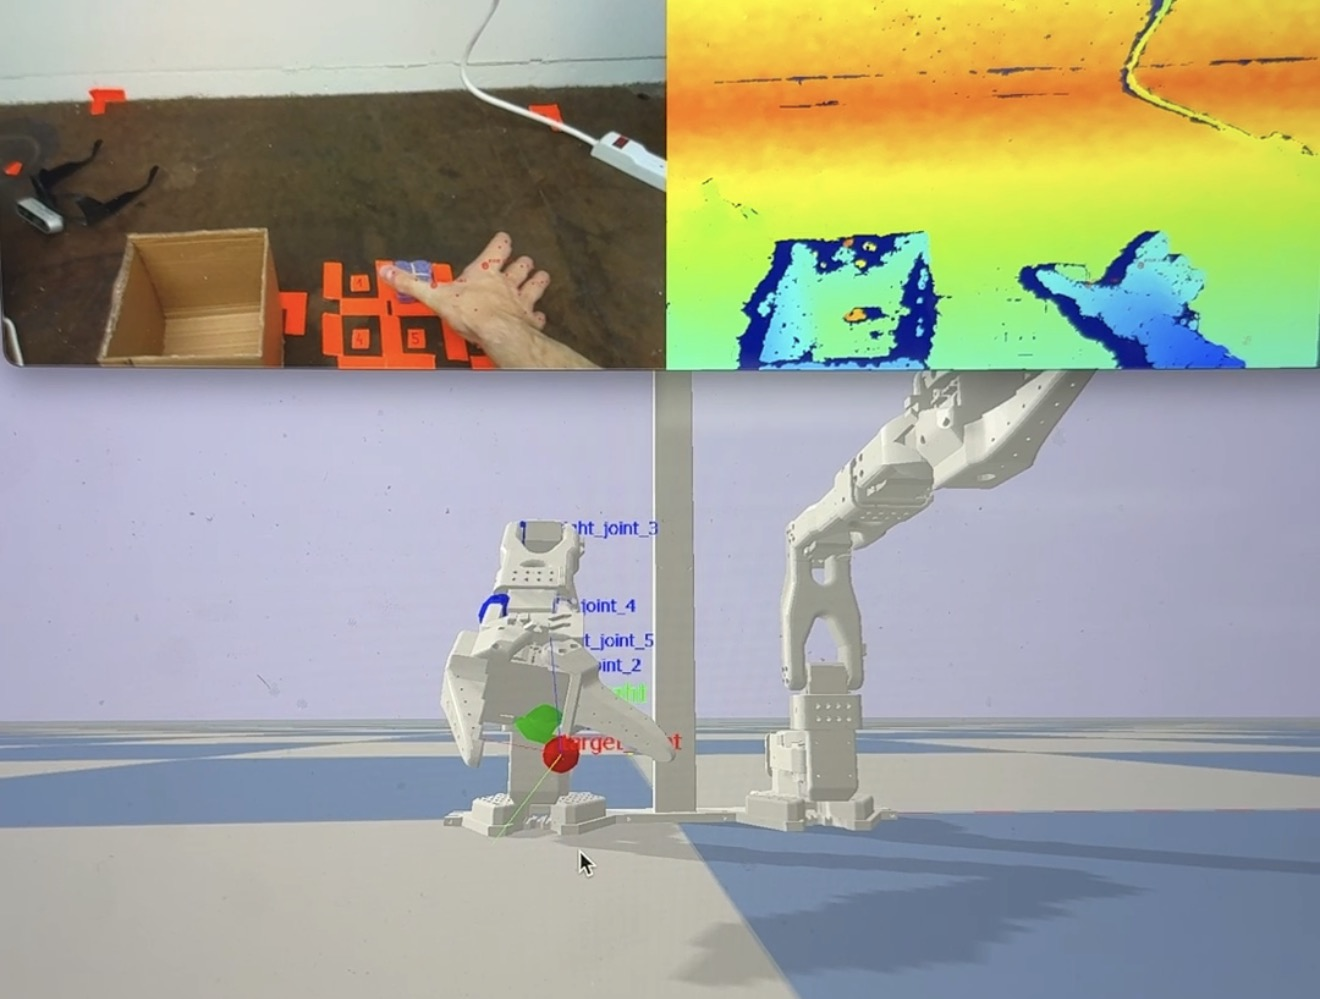
\includegraphics[width=0.9\columnwidth]{simulation.JPG}
\caption{\textbf{PyBullet simulation preview.} Top-left: RGB frame from the
  egocentric camera showing the operator's hand. Top-right: depth
  colour map. Bottom: robot arm in PyBullet with debug joint
  labels and IK target markers (green/red spheres), tracking the
  hand-derived trajectory.}
\label{fig:simulation}
\end{figure}

\subsection{Physical Deployment}
\label{sec:deployment}

Validated actions are deployed on the physical SO-ARM101 via the
LeRobot~\cite{lerobot2024} framework. Joint angles from the IK solver
(in radians) are normalised to $[0, 1]$ using the joint range
limits (Table~\ref{tab:joints}) and converted to motor commands:
\begin{equation}
  a_{\text{motor}} =
  \begin{cases}
    (a_{\text{norm}} - 0.5) \times 200 & \text{arm joints}, \\
    a_{\text{norm}} \times 100 & \text{gripper joint}.
  \end{cases}
\end{equation}

Servo PID coefficients are configured for smooth motion (Table~\ref{tab:servo}),
and acceleration/velocity limits prevent abrupt movements. Three gripper
modes are supported: \emph{Normal} (raw angle pass-through),
\emph{Binary} (threshold at $60^{\circ}$; outputs fully open or closed),
and \emph{Offset} (adds a configurable offset for tighter grasps).

Fig.~\ref{fig:shadowing} shows the hand-shadowing result:
the operator (left) grasps an object while wearing the camera glasses,
and the robot (right) mirrors the grasp posture via the
IK pipeline after offline processing.

\begin{figure}[t]
\centering
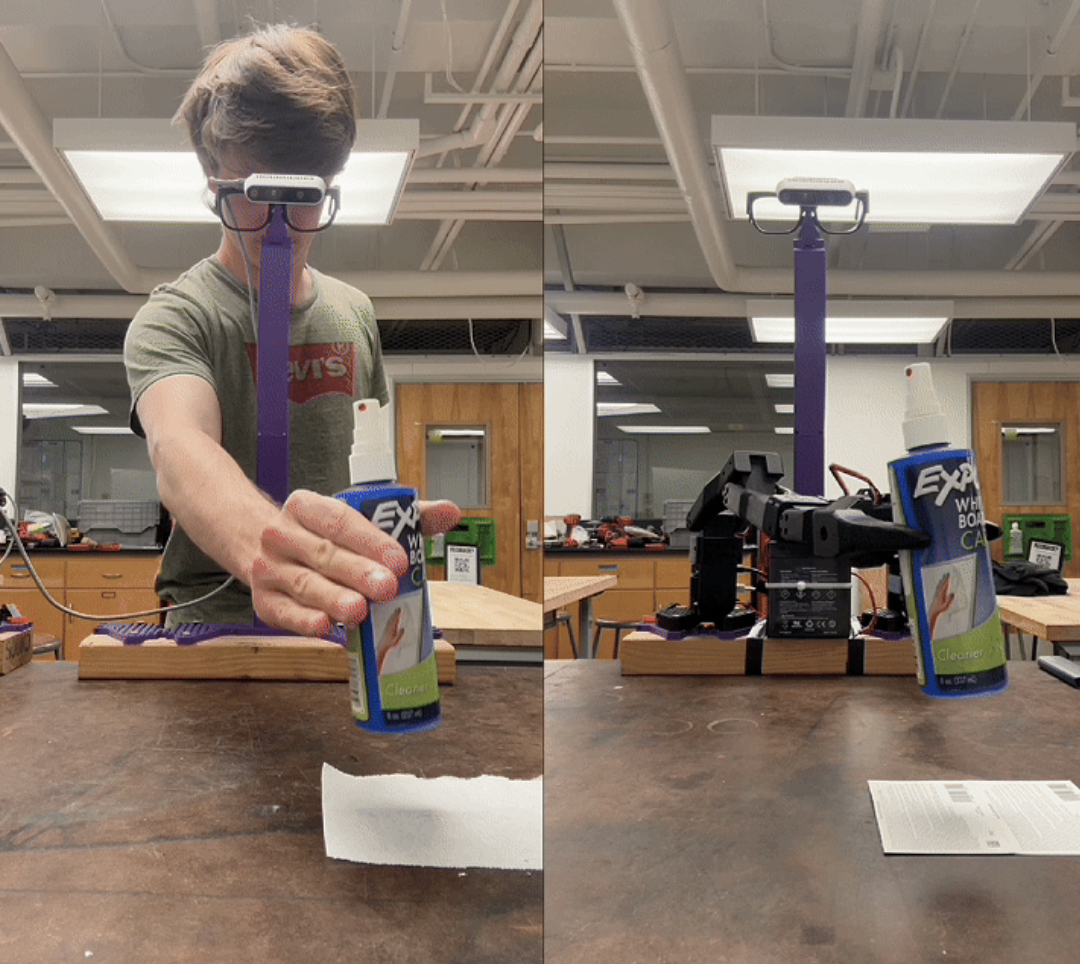
\includegraphics[width=0.9\columnwidth]{robot_shadowing_human_inrealtime.png}
\caption{\textbf{Hand shadowing.} Left: the operator wearing the
  RealSense glasses performs a grasp. Right: the SO-ARM101 robot
  mirrors the hand pose through the IK pipeline.}
\label{fig:shadowing}
\end{figure}

% ============================= 5  EXPERIMENTAL SETUP ========================
\section{Experimental Setup}
\label{sec:experiments}

\subsection{Hardware and Software}
\begin{itemize}
  \item \textbf{Camera}: Intel RealSense D400, 640$\times$480 RGB+D at 30\,FPS.
  \item \textbf{Robot}: Single SO-ARM101 follower arm (STS3215 servos,
        30\,kg$\cdot$cm torque).
  \item \textbf{Glasses}: Custom 3D-printed PLA mount (3 parts: frame,
        2$\times$ branch, mount bracket).
  \item \textbf{Compute}: Apple M-series or x86 laptop (MediaPipe runs
        on CPU; PyBullet IK requires no GPU).
  \item \textbf{Software}: Python 3.10, PyBullet $\geq$3.2.5,
        MediaPipe $\geq$0.10, LeRobot $\geq$0.4.1, OpenCV $\geq$4.8.
\end{itemize}

Table~\ref{tab:joints} lists the joint angle ranges that define the
normalisation bounds for physical deployment and the IK solver's
feasible set. Table~\ref{tab:servo} gives the servo PID and
motion-limit parameters.

\begin{table}[t]
\caption{\textbf{SO-ARM101 Joint Angle Ranges (Radians)}}
\label{tab:joints}
\centering
\begin{tabular}{lrrr}
\hline
\textbf{Joint} & \textbf{Min} & \textbf{Max} & \textbf{Range ($^{\circ}$)} \\
\hline
Shoulder pan   & $-1.920$ & $+1.920$ & $220.0$ \\
Shoulder lift  & $-1.745$ & $+1.745$ & $200.0$ \\
Elbow flex     & $-1.745$ & $+1.571$ & $190.0$ \\
Wrist flex     & $-1.658$ & $+1.658$ & $190.0$ \\
Wrist roll     & $-2.793$ & $+2.793$ & $320.0$ \\
Gripper        & $-0.175$ & $+1.745$ & $110.0$ \\
\hline
\end{tabular}
\end{table}

\begin{table}[t]
\caption{\textbf{Physical Robot Servo Parameters}}
\label{tab:servo}
\centering
\begin{tabular}{lr}
\hline
\textbf{Parameter} & \textbf{Value} \\
\hline
P coefficient               & 12 \\
I coefficient               & 0 \\
D coefficient               & 24 \\
Arm acceleration limit      & 50 / 254 \\
Gripper acceleration limit  & 100 / 254 \\
Arm velocity limit          & 1500\,RPM \\
Gripper velocity limit      & 3000\,RPM \\
\hline
\end{tabular}
\end{table}

\subsection{Task and Protocol}
\label{sec:task}

The benchmark task is: \emph{``Grab the purple cube and drop it in the
box.''} The cube is a soft foam block ($5 \times 5 \times 5$\,cm) placed
on a $3 \times 3$ tile grid (tiles numbered \#1--\#9), with a
$25 \times 25$\,cm cardboard box positioned to the left of the grid.
Fig.~\ref{fig:grabbing} shows the robot executing this task; the
tile grid is visible as orange tape markers on the bench surface.

For the IK pipeline, the operator wears the glasses and
performs the task naturally. The system records 30\,FPS RGB-D to a
\texttt{.bag} file, processes it offline to extract joint-angle actions,
previews the trajectory in PyBullet (Section~\ref{sec:simulation}),
and then deploys on the physical robot.

The reported benchmark uses tiles \#1--\#5 with 10 grasps per tile,
yielding $10 \times 5 = 50$ episodes per approach. Pilot trials on
tiles \#6--\#9 revealed two issues:
\begin{itemize}
  \item \textbf{IK pipeline}: tiles \#6--\#9 (closer to the robot base)
        require the operator to reach downward and behind, changing
        the hand orientation relative to the egocentric camera such
        that the thumb and index finger become partially self-occluded,
        preventing reliable gripper-angle computation.
  \item \textbf{VLA policies}: the robot's own gripper could occlude the
        cube in the policy input view at certain grid positions
        (discussed further in Section~\ref{sec:successrates}).
\end{itemize}
We therefore excluded tiles \#6--\#9 from the final evaluation.

\begin{figure}[t]
\centering
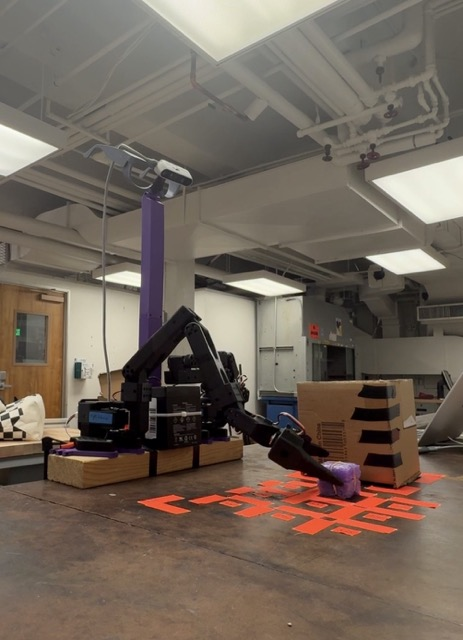
\includegraphics[width=0.9\columnwidth]{robot_grabbing_cube.JPG}
\caption{\textbf{Pick-and-place benchmark task.} The SO-ARM101 robot grasps
  the purple cube and places it in the box.
  The tile grid (\#1--\#9) is marked with orange tape; the box
  sits to the left. The RealSense camera is visible on the stand above.}
\label{fig:grabbing}
\end{figure}

\subsection{VLA Policy Training}
\label{sec:vlatraining}

For the imitation-learning comparison, 50 demonstration episodes
($\times$40\,s each, tiles \#1--\#5) are collected via
leader--follower teleoperation using a second SO-ARM101 as the leader
arm (standard LeRobot teleoperation setup) while the same external
RealSense camera records RGB and depth at 640$\times$480, 30\,FPS.
The demonstration data includes synchronised RGB, depth, and
joint-angle recordings, uploaded to the Hugging Face Hub
in LeRobot dataset format.

Four policies are fine-tuned on Google Colab (T4 GPU, 16\,GB):
\begin{itemize}
  \item \textbf{ACT}~\cite{zhao2023act}: batch size 4--6,
        50\,k steps. Learns a generative model over action chunks
        conditioned on image and proprioceptive observations.
  \item \textbf{SmolVLA}~\cite{cadena2025smolvla}: batch size 64,
        20\,k steps. A 450M-parameter vision-language-action model.
  \item \textbf{$\pi_{0.5}$}~\cite{black2024pi0}: batch size 32,
        3\,k steps, bfloat16. Fine-tuned from a pretrained VLM backbone.
  \item \textbf{GR00T~N1.5}: batch size 32, 3\,k steps. A
        cross-embodiment foundation model.
\end{itemize}

% ============================= 6  RESULTS ===================================
\section{Results and Discussion}
\label{sec:results}

\subsection{Pipeline Latency}

Fig.~\ref{fig:latency} shows the per-stage latency breakdown.
The three dominant stages are MediaPipe hand detection (23\,ms),
RGB/depth frame overlay and visualisation (110\,ms), and PyBullet
inverse kinematics solving (80\,ms). The total per-frame processing
time is $23 + 110 + 80 = 213$\,ms, yielding an effective throughput
of approximately ${\sim}$5\,FPS. The pipeline therefore
does \emph{not} operate in real time at the camera's native 30\,FPS:
frames are recorded to a \texttt{.bag} file at 30\,FPS, then processed
offline at ${\sim}$5\,FPS to produce joint-angle trajectories, which
are subsequently replayed on the robot at the target frame rate.

\begin{figure}[t]
\centering
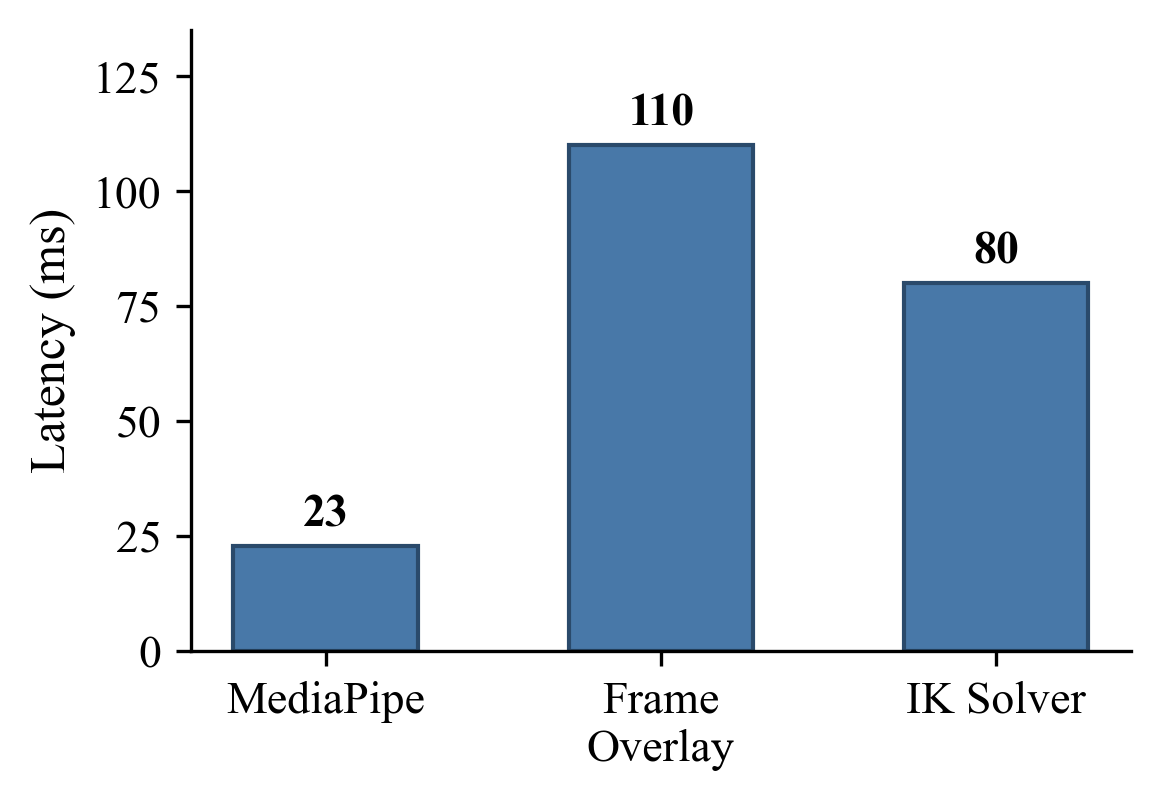
\includegraphics[width=0.85\columnwidth]{chart_latency.png}
\caption{\textbf{Per-stage latency breakdown.} The RGB/depth frame overlay
  (110\,ms) and PyBullet IK solver (80\,ms) dominate, yielding a
  total of 213\,ms per frame (${\sim}$5\,FPS). Processing is
  performed offline on recorded \texttt{.bag} files.}
\label{fig:latency}
\end{figure}

\subsection{Pick-and-Place Success Rates}
\label{sec:successrates}

Table~\ref{tab:successrates} reports the pick-and-place success rates
on tiles \#1--\#5 (50 episodes per approach, 10 grasps per tile).
The IK retargeting pipeline achieves a \textbf{90\%} success rate
(45/50) with zero training, since it analytically maps every operator
hand motion to the robot. Its failures stem exclusively from
thumb/index landmark detection issues at certain hand orientations,
which prevent the gripper angle from being computed (the four-level
fallback hierarchy recovers in most but not all cases).

Fig.~\ref{fig:pertile} shows the per-tile breakdown for the IK
pipeline. Tiles \#1 and \#2 (farthest from the robot, most natural
hand orientation) achieve 10/10 and 10/10 respectively. Success
degrades toward tile \#5 (closest to the robot base, requiring
downward hand orientation) at 7/10, consistent with the hand
self-occlusion failure mode identified in Section~\ref{sec:task}.

\begin{figure}[t]
\centering
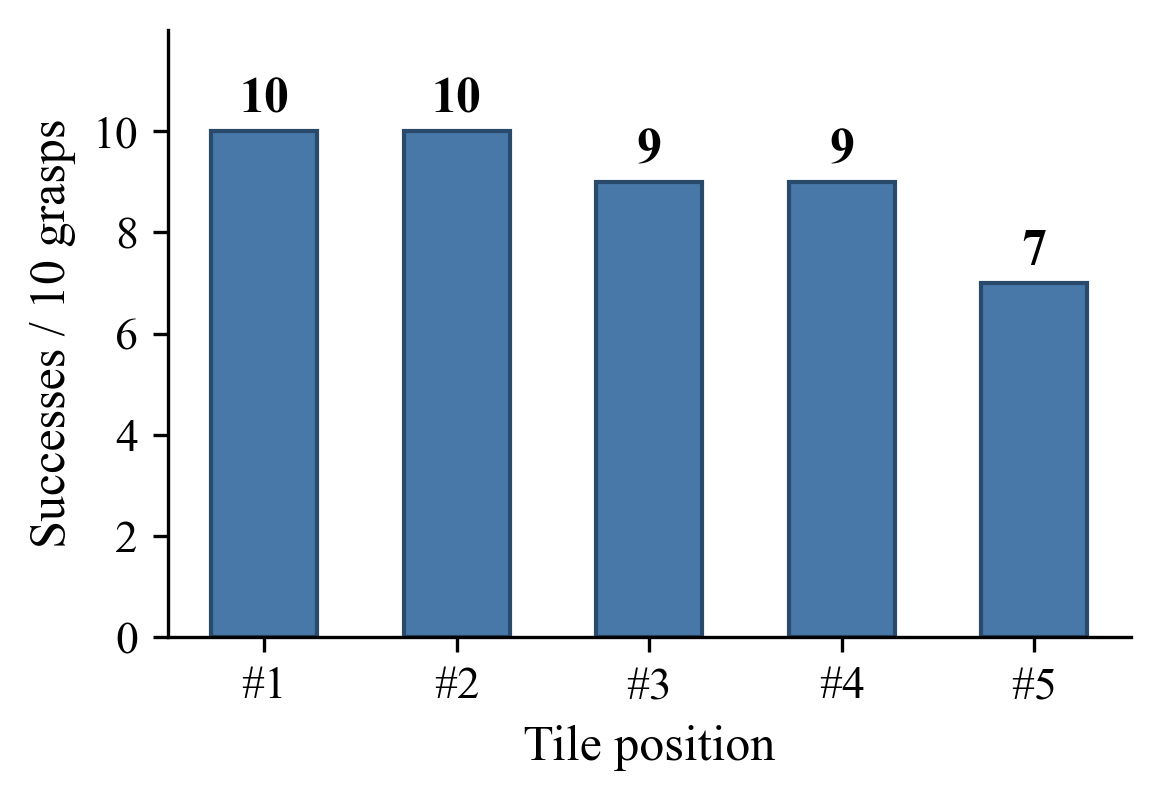
\includegraphics[width=0.85\columnwidth]{chart_pertile.png}
\caption{\textbf{IK retargeting per-tile success} (out of 10 grasps each).
  Tiles \#1--\#2 (farthest from robot, natural hand pose) achieve
  perfect scores. Performance degrades toward tile \#5 (closest
  to robot base) where the operator's hand orientation causes
  partial thumb/index self-occlusion from the egocentric camera.
  Total: 45/50 = 90\%.}
\label{fig:pertile}
\end{figure}

The four VLA policies are trained on 50 leader--follower teleoperation
episodes and evaluated on the same tile set. ACT achieves a
\textbf{92\%} success rate---slightly exceeding the IK pipeline. One
possible explanation is that leader--follower demonstrations provide
physically successful trajectories, whereas the IK pipeline must
reconstruct the motion from vision at every frame and can fail when
hand landmarks are poorly detected. ACT may also benefit from the
larger training budget (50\,k steps) on this structured task.
SmolVLA reaches 50\%, competitive
given its language-conditioning capability but limited by the
small number of training episodes. $\pi_{0.5}$ achieves 40\%, limited
by its short fine-tuning (3\,k steps) from the generalist pretrained
checkpoint. GR00T~N1.5 reaches 35\%, consistent with the challenge of
adapting a cross-embodiment foundation model to a specific low-cost arm.

A likely failure mode for SmolVLA, $\pi_{0.5}$, and GR00T~N1.5
is \emph{self-occlusion}: during the approach phase, the robot's
gripper can partially hide the cube in the camera view, reducing
visibility of the grasp target at a critical moment. ACT appears more
robust to this issue, possibly because action chunking can carry the
policy through short periods of occlusion, although this may also make
the policy more task-specific.

\begin{table}[t]
\caption{\textbf{Pick-and-Place Success Rates} (tiles \#1--\#5, 10 grasps
  per tile = 50 episodes). The IK pipeline requires no training; VLA
  policies are trained on leader--follower teleoperation demonstrations.}
\label{tab:successrates}
\centering
\begin{tabular}{lccr}
\hline
\textbf{Approach} & \textbf{Training} & \textbf{Inference} & \textbf{Success} \\
                   & \textbf{Steps}    & \textbf{Hz}        & \textbf{Rate} \\
\hline
IK Retargeting (ours) & ---           & ${\sim}$5 (offline) & 90\% \\
ACT~\cite{zhao2023act}          & 50\,k  & ${\sim}$10 & \textbf{92\%} \\
SmolVLA~\cite{cadena2025smolvla} & 20\,k  & ${\sim}$10 & 50\% \\
$\pi_{0.5}$~\cite{black2024pi0} & 3\,k   & ${\sim}$10 & 40\% \\
GR00T~N1.5            & 3\,k          & ${\sim}$10 & 35\% \\
\hline
\end{tabular}
\end{table}

\subsection{Approach Comparison}

Table~\ref{tab:comparison} compares the IK pipeline with the learned
policy approaches across key dimensions.

\begin{table}[t]
\caption{\textbf{Comparison of Teleoperation Approaches}}
\label{tab:comparison}
\centering
\begin{tabular}{p{1.8cm}p{1.4cm}p{3.5cm}}
\hline
\textbf{Property} & \textbf{IK (ours)} & \textbf{Learned Policies} \\
\hline
Training data
  & None
  & 50 episodes (33\,min) \\
Training time
  & 0
  & 2--8\,h on T4 GPU \\
Inference rate
  & ${\sim}$5\,Hz (offline)
  & ${\sim}$10\,Hz \\
Generalisation
  & Task-agnostic
  & Task-specific (ACT) or language-conditioned \\
Failure mode
  & Hand occlusion
  & Gripper self-occlusion \\
\hline
\end{tabular}
\end{table}

\subsection{In-the-Wild Evaluation}
\label{sec:inthewild}

To assess the generality of the IK retargeting approach beyond the
structured lab bench, we deployed the system in two unstructured
real-world environments: a grocery store and a pharmacy. The robot and
supporting compute setup were placed on a standard shopping basket,
which provides a repeatable height across trials and positions the
robot arm within ${\sim}$30\,cm of shelf objects---a necessary
constraint since the human arm (${\sim}$60\,cm reach) is significantly
longer than the SO-ARM101 (${\sim}$30\,cm reach).

Fig.~\ref{fig:inthewild_setup} shows the in-the-wild setup: the
operator, still wearing the glasses-mounted camera, reaches for items
on the store shelf (left) while the robot
mounted in the shopping basket reproduces the motion via IK retargeting
after offline processing (right). The task involves grasping various
store items (cans, bottles, boxes) from the shelf and placing them in
the basket.

Over 75 grasp attempts across both locations, only 7 succeeded,
yielding a success rate of \textbf{9.3\%}.

The primary failure mode is \emph{hand occlusion by surrounding
objects}: in a cluttered shelf environment, the operator's hand is
frequently occluded by adjacent products, shelf edges, and price tags
from the egocentric camera's perspective. This causes MediaPipe to lose
track of the thumb and index finger landmarks, preventing both the
gripper angle computation and the IK target position calculation.

Despite the low overall success rate, the 7 successful grasps---shown
in the mosaic in Fig.~\ref{fig:inthewild_mosaic}---indicate that the
pipeline can transfer to unstructured environments when hand visibility
is preserved, suggesting that occlusion handling is a key area for
improvement.

\begin{figure}[t]
\centering
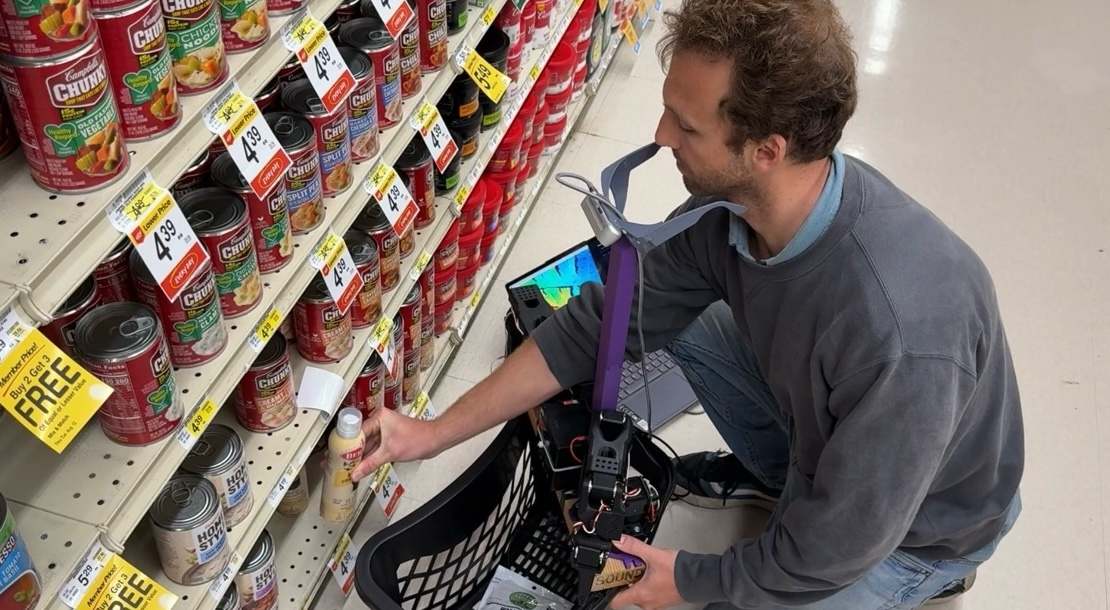
\includegraphics[width=0.48\columnwidth]{inthewild_humanhandhandcapture.JPG}
\hfill
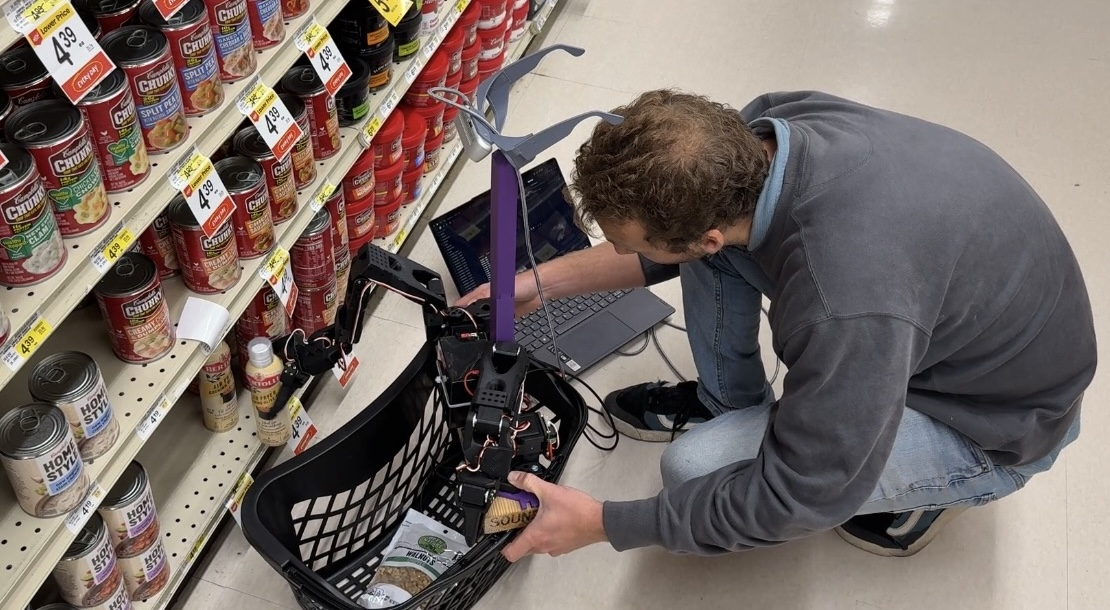
\includegraphics[width=0.48\columnwidth]{inthewild_robotIK.JPG}
\caption{\textbf{In-the-wild deployment in a grocery store.} The robot and
  supporting compute setup are placed on a shopping basket for
  repeatable height. Left: the operator reaches for shelf items while
  wearing the glasses-mounted camera.
  Right: the robot mirrors the motion; the PyBullet preview is visible
  on the laptop screen.}
\label{fig:inthewild_setup}
\end{figure}

\begin{figure}[t]
\centering
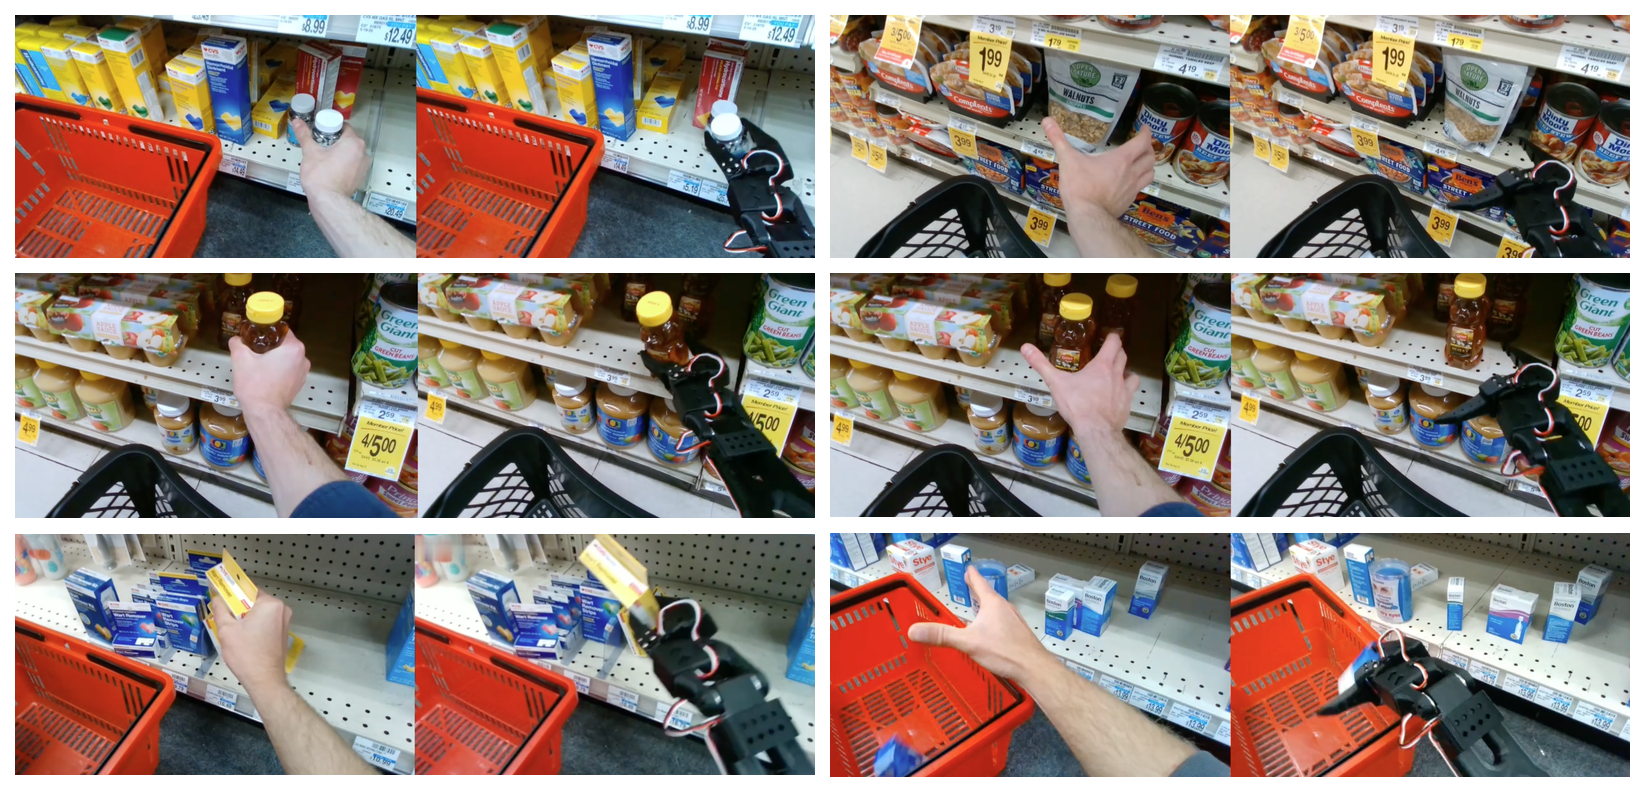
\includegraphics[width=0.9\columnwidth]{mosaic_in_the_wild.png}
\caption{\textbf{Mosaic of successful in-the-wild grasps} (7 out of 75
  attempts). Each pair shows the human hand capture (left) and the
  corresponding robot IK retargeting (right) for various store items
  across grocery and pharmacy environments. Despite an overall 9.3\%
  success rate, successful transfers demonstrate the pipeline's
  potential in unstructured scenes.}
\label{fig:inthewild_mosaic}
\end{figure}

\subsection{Failure Modes}

We identify the following primary failure modes, separated by context.

\subsubsection{Structured Lab Environment}
\begin{enumerate}
  \item \textbf{Thumb/index detection failure}: At certain hand
        orientations (particularly toward tiles
        \#6--\#9), the thumb and index finger landmarks are poorly
        detected, preventing gripper angle computation. This is the
        dominant IK failure mode (accounting for all 10\% of lab
        failures).
  \item \textbf{Gripper self-occlusion (VLAs)}: The robot's gripper
        can hide the cube in the camera view during the approach
        phase. This effect appears most pronounced for SmolVLA,
        $\pi_{0.5}$, and GR00T~N1.5, where the vision model loses
        sight of the grasp target at a critical moment.
  \item \textbf{Gripper jitter}: Rapid open-close oscillations occur
        when the thumb-index angle is near the binary threshold. The
        binary gripper mode with a $60^{\circ}$ threshold resolves this.
\end{enumerate}

\subsubsection{Unstructured In-the-Wild Environments}
\begin{enumerate}
  \item \textbf{Hand occlusion by scene objects}: Shelf products,
        price tags, and adjacent items frequently occlude the
        operator's hand from the egocentric camera, causing MediaPipe
        to lose landmark tracking. This is the dominant failure mode,
        accounting for the drop from 90\% to 9.3\% success.
  \item \textbf{Workspace mismatch}: The human arm (${\sim}$60\,cm)
        reaches further than the robot (${\sim}$30\,cm), requiring
        careful positioning of the shopping basket to keep objects
        within the robot's reachable volume.
  \item \textbf{Depth noise}: Reflective packaging (foil, plastic
        wrap) produces unreliable depth readings, causing spurious
        3D deprojection results.
\end{enumerate}

% ============================= 7  CONCLUSION ================================
\section{Conclusion}

We have presented a vision-based hand-shadowing system for
offline robot trajectory generation via egocentric hand tracking and
analytical inverse kinematics. The pipeline processes recorded RGB-D frames at
${\sim}$5\,FPS (213\,ms per frame) using MediaPipe Hands for landmark
detection, depth-based 3D deprojection, and PyBullet for IK solving
and trajectory preview, with the LeRobot framework for physical
deployment on the SO-ARM101.

On a structured pick-and-place benchmark (tiles \#1--\#5, 50 episodes),
the IK retargeting pipeline achieves 90\% success with zero training.
Among the teleoperation-trained VLA policies, ACT reaches 92\%, while
SmolVLA (50\%), $\pi_{0.5}$ (40\%), and GR00T~N1.5 (35\%) are
substantially lower. The gap is consistent with the structured nature
of the benchmark and with visibility challenges caused by gripper
self-occlusion in the camera view.
In-the-wild evaluation in grocery store and pharmacy environments
(7/75 successful grasps, 9.3\%) indicates that hand occlusion by
surrounding objects is the primary limitation of the current system.

\subsection{Future Work}
\begin{itemize}
  \item \textbf{Occlusion-robust hand tracking}: Temporal hand tracking,
        learned depth completion, or multi-camera setups to maintain
        landmark visibility in cluttered environments.
  \item \textbf{Dual-arm extension}: The current system controls a
        single arm; extending to simultaneous bimanual control.
  \item \textbf{IK demonstrations for VLA training}: Using IK-collected
        trajectories as training data for VLA policies, potentially
        avoiding the gripper self-occlusion issue present in
        leader--follower teleoperation data.
  \item \textbf{Larger workspace}: Adaptive camera-to-robot calibration
        for dynamic operator positioning.
  \item \textbf{Force feedback}: Integrating gripper force sensing for
        haptic feedback to the operator.
\end{itemize}

\section*{Acknowledgment}
The authors thank the UC Berkeley Department of Mechanical Engineering
and the Fung Institute for Engineering Leadership for providing
access to lab facilities, equipment, and student collaboration.

\begin{thebibliography}{00}

\bibitem{potamias2024wilor}
R.~A. Potamias, J.~Zhang, J.~Deng, and S.~Zafeiriou,
``WiLoR: End-to-end 3D hand localization and reconstruction in-the-wild,''
\emph{arXiv preprint arXiv:2409.12259}, 2024.

\bibitem{zhang2020mediapipe}
F.~Zhang, V.~Bazarevsky, A.~Vakunov, A.~Tkachenka, G.~Sung, C.-L.~Chang,
and M.~Grundmann,
``MediaPipe Hands: On-device real-time hand tracking,''
\emph{arXiv preprint arXiv:2006.10214}, 2020.

\bibitem{romero2017mano}
J.~Romero, D.~Tzionas, and M.~J. Black,
``Embodied hands: Modeling and capturing hands and bodies together,''
\emph{ACM Trans. Graphics (Proc. SIGGRAPH Asia)},
vol.~36, no.~6, pp.~245:1--245:17, 2017.

\bibitem{zhao2023act}
T.~Z. Zhao, V.~Kumar, S.~Levine, and C.~Finn,
``Learning fine-grained bimanual manipulation with low-cost hardware,''
\emph{arXiv preprint arXiv:2304.13705}, 2023.

\bibitem{cadena2025smolvla}
F.~Cadena \emph{et al.},
``SmolVLA: A vision-language-action model for affordable and efficient
robotics,''
\emph{arXiv preprint arXiv:2506.01844}, 2025.

\bibitem{black2024pi0}
K.~Black \emph{et al.},
``$\pi_0$: A vision-language-action flow model for general robot control,''
\emph{arXiv preprint arXiv:2410.24164}, 2024.

\bibitem{cheng2025opentv}
X.~Cheng \emph{et al.},
``Open-TeleVision: Teleoperation with immersive active visual feedback,''
in \emph{Proc. CoRL}, 2025.

\bibitem{ding2024bunny}
Y.~Ding \emph{et al.},
``Bunny-VisionPro: Real-time bimanual dexterous teleoperation for
imitation learning,''
\emph{arXiv preprint arXiv:2407.03162}, 2024.

\bibitem{keselman2017realsense}
L.~Keselman, J.~I. Woodfill, A.~Grunnet-Jepsen, and A.~Bhowmik,
``Intel RealSense stereoscopic depth cameras,''
in \emph{Proc. CCD Workshop, CVPR}, 2017.

\bibitem{coumans2021pybullet}
E.~Coumans and Y.~Bai,
``PyBullet, a Python module for physics simulation for games, robotics
and machine learning,''
\url{http://pybullet.org}, 2016--2021.

\bibitem{lerobot2024}
Hugging Face,
``LeRobot: State-of-the-art machine learning for real-world robotics,''
\url{https://github.com/huggingface/lerobot}, 2024.

\bibitem{soarm100}
The Robot Studio,
``SO-ARM100: Open-source 6-DOF robotic arm,''
\url{https://github.com/TheRobotStudio/SO-ARM100}, 2024.

\end{thebibliography}

\end{document}
